\documentclass[../main]{subfiles}

\begin{document}
\section{Numerical experiments} \zlabel{sec:acc_pgm:experiments}
This section compares the performance of \zcref{alg:acc_pgm_MO} with various~$a$ and~$b$ through numerical experiments.
We run all experiments in Python 3.9.9 on a machine with 2.3 GHz Intel Core i7 CPU and 32 GB memory.
For each example, we test 15 different hyperparameters combining~$a = 0, 1 / 6, 1 / 4, 1 / 2, 3 / 4$ and~$b = a^2 / 4, (a^2 + 1) / 8, 1 / 4$, i.e.,
\begin{equation}
    (a, b) = \left\{
        \begin{gathered}
            (0, 0), (0, 1 / 8), (0, 1 / 4),\\
            (1 / 6, 1 / 144), (1 / 6, 37 / 288), (1 / 6, 1 / 4),\\
            (1 / 4, 1 / 64), (1 / 4, 17 / 128), (1 / 4, 1 / 4), \\
            (1 / 2, 1 / 16), (1 / 2, 5 / 32), (1 / 2, 1 / 4), \\
            (3 / 4, 9 / 64), (3 / 4, 25 / 128), (3 / 4, 1 / 4)
        \end{gathered}
    \right\},
\end{equation} 
and we set~$\varepsilon = 10^{-5}$ for the stopping criteria.

\subsection{Artificial test problems (bi-objective and tri-objective)}
First, we solve the multi-objective test problems in the form~\zcref{eq:MOO}, modifications from~\cite{Jin2001,Fliege2009}, whose objective functions are defined by
\begin{align}
    &f_1(x) = \frac{1}{n} \norm*{x}_2^2,
    f_2(x) = \frac{1}{n} \norm*{x - 2}_2^2,
    g_1(x) = g_2(x) = 0, \tag{JOS1}\label{eq:JOS1} \\
    &\left\{
        \begin{aligned}
            f_1(x) &= \frac{1}{n} \norm*{x}_2^2,
            f_2(x) = \frac{1}{n} \norm*{x - 2}_2^2, \\
            g_1(x) &= \frac{1}{n} \norm*{x}_1,
            g_2(x) = \frac{1}{2n} \norm*{x - 1}_1,
        \end{aligned} \right.
        \label{eq:JOS1_L1} \tag{JOS1-L1}\\
    &\left\{\begin{aligned} 
            f_1(x) &= \frac{1}{n^2} \sum_{i = 1}^{n} i (x_i - i)^4,
            f_2(x) = \exp \left( \sum_{i = 1}^{n} \frac{x_i}{n} \right) + \norm*{x}_2^2,\\
            f_3(x) &= \frac{1}{n (n + 1)} \sum_{i = 1}^{n} i (n - i + 1) \exp (- x_i),
            g_1(x) = g_2(x) = g_3(x) = 0,
    \end{aligned} \right. \label{eq:FDS} \tag{FDS}\\
    &\left\{\begin{aligned} 
            f_1(x) &= \frac{1}{n^2} \sum_{i = 1}^{n} i (x_i - i)^4,
            f_2(x) = \exp \left( \sum_{i = 1}^{n} \frac{x_i}{n} \right) + \norm*{x}_2^2,\\
            f_3(x) &= \frac{1}{n (n + 1)} \sum_{i = 1}^{n} i (n - i + 1) \exp (- x_i),
            g_1(x) = g_2(x) = g_3(x) = \indicator_{\setRpos^n}(x),
    \end{aligned} \right.\label{eq:FDS_CONSTRAINED} \tag{FDS-CON}
\end{align}
where~$x \in \setR^n, n = 50$ and~$\indicator_{\setRpos^n}$ is an indicator function~\zcref{eq:indicator} of the nonnegative orthant.
We choose~$1000$ initial points, commonly for all pairs~$(a, b)$, and randomly with a uniform distribution between~$\underline{c}$ and~$\overline{c}$, where~$\underline{c} = (-2, \dots, -2)^\T$ and~$\overline{c} = (4, \dots, 4)^\T$ for~\zcref{eq:JOS1,eq:JOS1_L1},~$\underline{c} = (-2, \dots, -2)^\T$ and~$\overline{c} = (2, \dots, 2)^\T$ for~\zcref{eq:FDS}, and~$\underline{c} = (0, \dots, 0)^\T$ and~$\overline{c} = (2, \dots, 2)^\T$ for~\zcref{eq:FDS_CONSTRAINED}.
Moreover, we use backtracking for updating~$\alpha$ to satisfy~\zcref{eq:acc_pgm_sdc}, with~$1$ as the initial value of~$\alpha$ and~$0.5$ as the constant multiplied into~$\alpha$ at each iteration.
Furthermore, at each iteration, we transform the subproblem~\zcref{eq:acc_pgm_subprob} into their dual like~\zcref{eq:dual_reg_lin_gap} and solve them with the trust-region interior point method~\cite{Byrd1999} using the scientific library SciPy.

\zcref{fig:Pareto,tab:Average computational costs} present the experimental results.
\zcref{fig:Pareto} plots the solutions only for the cases~$(a, b) = (0, 1 / 4), (3 / 4, 1 / 4)$, but other combinations also yield similar plots, including a wide range of Pareto solutions.
\zcref{tab:Average computational costs} shows that the new momentum factors are fast enough to compete with the existing ones ($(a, b) = (0, 1/4)$ or $b = a^2/4$) and better than them in some cases.

\begin{figure}[htbp]
    \centering
    \begin{minipage}[b]{.49\hsize}
        \centering
        \begin{minipage}[b]{.49\hsize}
            \centering
            \adjincludegraphics[trim={{.66\width} {.8\height} 0 0}, clip, width=\linewidth]{figs/JOS1_ab.pdf}
        \end{minipage}
        \begin{minipage}[b]{.49\hsize}
            \centering
            \adjincludegraphics[trim={{.66\width} 0 0 {.8\height}}, clip, width=\linewidth]{figs/JOS1_ab.pdf}
        \end{minipage}
        \subcaption{\zcref{eq:JOS1}}
        \zlabel{fig:JOS1}
    \end{minipage}
    \begin{minipage}[b]{.49\hsize}
        \centering
        \begin{minipage}[b]{.49\hsize}
            \centering
            \adjincludegraphics[trim={{.66\width} {.8\height} 0 0}, clip, width=\linewidth]{figs/JOS1_L1_ab.pdf}
        \end{minipage}
        \begin{minipage}[b]{.49\hsize}
            \centering
            \adjincludegraphics[trim={{.66\width} 0 0 {.8\height}}, clip, width=\linewidth]{figs/JOS1_L1_ab.pdf}
        \end{minipage}
        \subcaption{\zcref{eq:JOS1_L1}}
        \zlabel{fig:JOS1_L1}
    \end{minipage}
    \begin{minipage}[b]{.49\hsize}
        \centering
        \begin{minipage}[b]{.49\hsize}
            \centering
            \adjincludegraphics[trim={{.605\width} {.8\height} {.014\width} 0}, clip, width=\linewidth]{figs/FDS_ab.pdf}
        \end{minipage}
        \begin{minipage}[b]{.49\hsize}
            \centering
            \adjincludegraphics[trim={{.605\width} 0 {.014\width} {.8\height}}, clip, width=\linewidth]{figs/fDS_ab.pdf}
        \end{minipage}
        \subcaption{\zcref{eq:FDS}}
        \zlabel{fig:FDS}
    \end{minipage}
    \begin{minipage}[b]{.49\hsize}
        \centering
        \begin{minipage}[b]{.49\hsize}
            \centering
            \adjincludegraphics[trim={{.605\width} {.8\height} {.014\width} 0}, clip, width=\linewidth]{figs/FDS_CONSTRAINED_ab.pdf}
        \end{minipage}
        \begin{minipage}[b]{.49\hsize}
            \centering
            \adjincludegraphics[trim={{.605\width} 0 {.014\width} {.8\height}}, clip, width=\linewidth]{figs/FDS_CONSTRAINED_ab.pdf}
        \end{minipage}
        \subcaption{\zcref{eq:FDS_CONSTRAINED}}
        \zlabel{fig:FDS_CON}
    \end{minipage}
    \caption{Pareto solutions obtained with some~$(a, b)$}
    \zlabel{fig:Pareto}
\end{figure}
\begin{table}[htbp]
    \centering
    \caption{Average computational costs to solve the multi-objective examples}
    \zlabel{tab:Average computational costs}
    \begin{minipage}{.49\hsize}
        \centering
        \subcaption{\zcref{eq:JOS1}}
        \begin{tabular}{@{}cccc@{}}
            \toprule
            $a$ & $b$ & Time [\si{\second}] & Iterations \\
            \midrule
        \csvreader[no head,late after line=\\]{data/JOS1_ab.csv}
        {1=\a, 2=\b,3=\totaltime,4=\iterationcounts}
            { $\a$ & $\b$ & \totaltime & \iterationcounts}
            \midrule
        \end{tabular}
    \end{minipage}
    \begin{minipage}{.49\hsize}
        \centering
        \subcaption{\zcref{eq:JOS1_L1}}
        \begin{tabular}{@{}cccc@{}}
            \toprule
            $a$ & $b$ & Time [\si{\second}] & Iterations \\
            \midrule
        \csvreader[no head,late after line=\\]{data/JOS1_L1_ab.csv}
        {1=\a, 2=\b,3=\totaltime,4=\iterationcounts}
            { $\a$ & $\b$ & \totaltime & \iterationcounts}
            \bottomrule
        \end{tabular}
    \end{minipage}
    \begin{minipage}{.49\hsize}
        \centering
        \subcaption{\zcref{eq:FDS}}
        \begin{tabular}{@{}cccc@{}}
            \toprule
            $a$ & $b$ & Time [\si{\second}] & Iterations \\
            \midrule
        \csvreader[no head,late after line=\\]{data/FDS_ab.csv}
        {1=\a, 2=\b,3=\totaltime,4=\iterationcounts}
            { $\a$ & $\b$ & \totaltime & \iterationcounts}
            \bottomrule
        \end{tabular}
    \end{minipage}
    \begin{minipage}{.49\hsize}
        \centering
        \subcaption{\zcref{eq:FDS_CONSTRAINED}}
        \begin{tabular}{@{}cccc@{}}
            \toprule
            $a$ & $b$ & Time [\si{\second}] & Iterations \\
            \midrule
        \csvreader[no head,late after line=\\]{data/FDS_CONSTRAINED_ab.csv}
        {1=\a, 2=\b,3=\totaltime,4=\iterationcounts}
            { $\a$ & $\b$ & \totaltime & \iterationcounts}
            \bottomrule
        \end{tabular}
    \end{minipage}
\end{table}

\subsection{Image deblurring (single-objective)}
Since our proposed momentum factor is also new in the single-objective context, we also tackle deblurring the cameraman test image via a single-objective $\ell_2$-$\ell_1$ minimization, inspired by~\cite{Beck2009}.
In detail, as shown in \zcref{fig:cameraman}, to a~$256 \times 256$ cameraman test image with each pixel scaled to~$[0,1]$, we generate an observed image by applying a Gaussian blur of size~$9 \times 9$ and standard deviation $4$ and adding a zero-mean white Gaussian noise with standard deviation $10^{-3}$.
\begin{figure}[htpb]
    \centering
    \begin{minipage}[b]{.45\hsize}
        \centering
        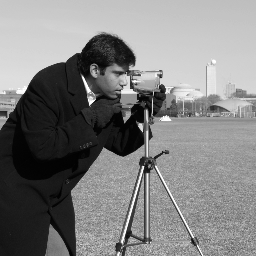
\includegraphics[width=0.8\textwidth]{figs/cameraman_original.png}
        \subcaption{Original}
        \zlabel{fig:cameraman:original}
    \end{minipage}
    \begin{minipage}[b]{.45\hsize}
        \centering
        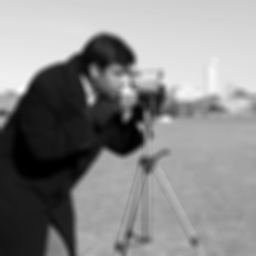
\includegraphics[width=0.8\textwidth]{figs/cameraman_blurred_and_noisy.png}
        \subcaption{Blurred and noisy}
        \zlabel{fig:cameraman:blurred_and_noisy}
    \end{minipage}
    \caption{Deblurring of the cameraman}
    \zlabel{fig:cameraman}
\end{figure}

Letting~$\theta, B,$ and~$W$ be the observed image, the blur matrix, and the inverse of the Haar wavelet transform, respectively, consider the single-objective problem~\zcref{eq:MOO} with~$m = 1$ and
\begin{equation} \label{eq:cam_deblur} \tag{CAM-DEBLUR}
    f_1(x) \coloneqq \norm*{BWx - \theta}_2^2 \eqand g_1(x)=\lambda \norm*{x}_1
,\end{equation} 
where~$\lambda \coloneqq 2 \times 10^{-5}$ is a regularization parameter.
Unlike in the previous subsection, we can compute~$\nabla f$'s Lipschitz constant by calculating~$(BW)^\T(BW)$'s eigenvalues using the two-dimensional cosine transform~\cite{Hansen2006}, so we use it constantly as~$\alpha^{-1}$.
Moreover, we use the observed image's Wavelet transform as the initial point.

\zcref{fig:deblurred} shows the reconstructed image from the obtained solution.
Images produced by all hyperparameters are similar, so we present only~$(a, b) = (0, 1 / 4)$ and~$(1 / 2, 1 / 4)$.
Moreover, we summarize the numerical performance in \zcref{tab:cam_deblur,fig:cameraman_plot}.
Like the last subsection, this example suggests that our new momentum factors may occasionally improve the algorithm's performance even for single-objective problems.

\begin{figure}[htpb]
    \centering
    \begin{minipage}[b]{.49\hsize}
        \centering
        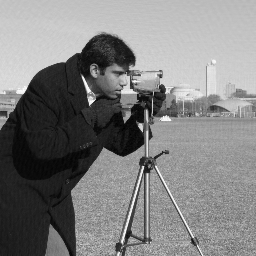
\includegraphics[width=\linewidth]{figs/cameraman_deblurred_2.png}
        \subcaption{$(a, b) = (0 , 1 / 4)$}
    \end{minipage}
    \begin{minipage}[b]{.49\hsize}
        \centering
        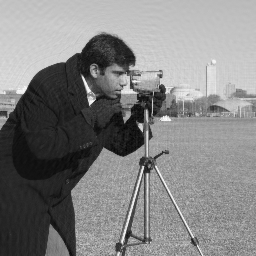
\includegraphics[width=\linewidth]{figs/cameraman_deblurred_11.png}
        \subcaption{$(a, b) = (1 / 2, 1 / 4)$}
    \end{minipage}
    \caption{Deblurred image}
    \zlabel{fig:deblurred}
\end{figure}

\begin{table}[htbp]
    \centering
    \caption{Computational costs for the image deblurring}
    \zlabel{tab:cam_deblur}
    \begin{tabular}{@{}cccc@{}}
        \toprule
         $a$ & $b$ & Total time [\si{\second}] & Iteration counts \\
        \midrule
    \csvreader[no head,late after line=\\]{data/cameraman_ab.csv}
    {1=\a, 2=\b,3=\totaltime,4=\iterationcounts}
        { $\a$ & $\b$ & \totaltime & \iterationcounts}
       \bottomrule
    \end{tabular}
\end{table}

\begin{figure}[htpb]
    \centering
    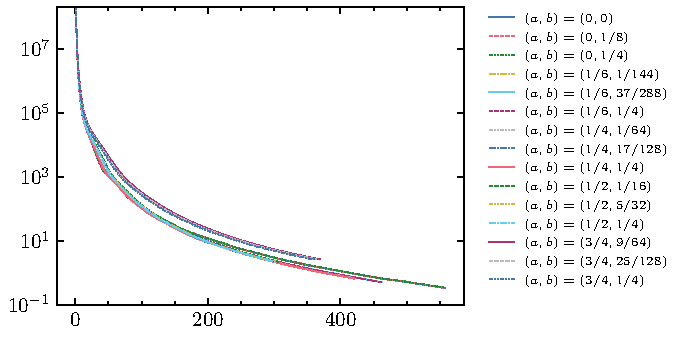
\includegraphics[width=\textwidth]{figs/cameraman_plot.pdf}
    \caption{Values of~$u_\infty\left(x^k\right) = F_1(x) - F_1(x^\ast)$, where~$x^\ast$ is the optimal solution estimated from the original image}
    \zlabel{fig:cameraman_plot}
\end{figure}

\end{document}
